% v0.2
% - Introduction section added
% - typos revised
% - 


\documentclass{easychair}
\usepackage{graphicx}
\usepackage{caption}
\usepackage{listings}
\usepackage{algpseudocode}
\usepackage{algorithm} 
\usepackage{amsmath}
\usepackage[font=footnotesize]{subcaption}
\usepackage{bsymb}
\usepackage{color,bcode,%citesort,
pb-diagram}
\setcounter{secnumdepth}{3}
\setmainfont{Hoefler Text}

% working with <let> keyword in algpseudocode
\newcommand*\Let[2]{\State #1 $\gets$ #2}
\algrenewcommand{\algorithmicforall}{\textbf{for each}}
\def\ForEach{\ForAll}

\newenvironment{keywords}{
       \list{}{\advance\topsep by0.35cm\relax\small
       \leftmargin=1cm
       \labelwidth=0.35cm
       \listparindent=0.35cm
       \itemindent\listparindent
       \rightmargin\leftmargin}\item[\hskip\labelsep
                                     \bfseries Keywords:]}
     {\endlist}
     
\begin{document}
\pagestyle{plain}
\pagenumbering{arabic}

\title{Automated Translation from Event-B specifications to Recursive Algorithms
\\\small{- 21/10/2013 - ver.0.2} 
}
\author{
Zheng Cheng \and
Rosemary Monahan 
}

\institute{
Computer Science Department\\
National University of Ireland Maynooth\\
Co. Kildare, Ireland\\
}

\maketitle  

\begin{abstract}
Event-B is a modelling language. It allows the user to develop software or algorithm in a step-by-step manner, i.e. refining an inital high level specification into a final concrete specification. In previous work, one of the author and her collegue decribes an approach that translating the final concrete specification into recursive and iterative implementation. In this document, we provide technical details of how the translation is performed. Moreover, we interest in the visualization of recursive algorithm for better readability and understandability.
 
\end{abstract}   

\begin{keywords}
 Event-B,
 Recursive Algorithm
\end{keywords}

\section{Introduction} % [ZHENG 21/10/2013] Newly added from v0.0
Event-B is a formal modelling language, based on refinement calculas. It uses set theory as a modelling notation, and use refinement to represent software systems at different abstraction levels. The use of mathematical proof will verify consistency between refinement levels.

Rodin platform is a tool set that help orgnize the information for systems written in Event-B. In addition, it provides theroem proving facilities that allow mathematical proofs to be semi-automatically discharged.

An Event-B model consists of the $contexts$ and $machines$. The $contexts$ give static information about the model, which will be refered in the machines. The machines express dynamic information about the model via $events$, which modify state variables and cause the model moving into a particular state. Optionally, the machine can express other properties, such as invariant and safty properties of the model.

Each event is triggered by conditions (i.e. $guards$) to take $actions$. When the Event-B model is in a state that satifies all the guards of an event, such event will take effect by performing defined actions.

% [ZHENG 21/10/2013] Might be an example of Evnet-B model with control variable? 
The control variable is an mechanism to control how the events interact with each other\ref{}. The user defines a set of control labels in the context, and declare a state variable (namely the control variable) in the machine to refer these labels. The control variable does not serve any purposes to the state of Event-B model. It only keeps track of an implicit control flow of the Event-B model. More specifically, if an event's guard refer to the control variable, it implies which events that lead to the current event. If an event's actions refer to the control variable, it suggests which events the current event can move into. 

In this document, we draw on the control variable mechanism in Event-B model, and present a plugin that read in an Event-B model to produce recursive algorithm and its visualized representation.
 
\section{The Translation Procedure}
To allow our plug-in understand that how to process an Event-B machine, the user needs to define a configuration file. This configuration file should specify at least:
\begin{itemize}
	\item The method signature under consideration.
	\item The name of the control variable (a.k.a label).
	\item The name of the start label.
\end{itemize}

Our plugin reads in the configuration file and starts to process the Event-B machine. To reduce the translation complexity from a Event-B machine to its corresponding recursive algorithm, the plug-in extracts required information out of each event in the original Event-B machine, and stores it in a data structure called \textbf{bEventObject} (see Fig~\ref{fig:ebo}). 

\begin{figure}[!h]
  \centering
    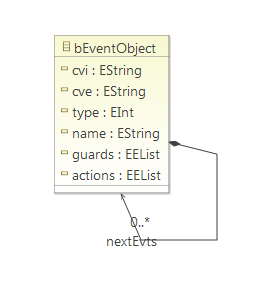
\includegraphics[width=0.5\textwidth]{img/ebo.PNG}
  \caption{The Data Structure of bEventObject}
  \label{fig:ebo}
\end{figure}

%Def 1.
The bEventObject is a 7-tuple $E_o = (cvi, cve, type, name, guards, actions, nextEvts)$, which consists of:
\begin{itemize}
	\item The initial control variable (cvi).
	\item The end control variable (cve).
	\item The type of the event (type).
	\item The name of the event (name).
	\item A set of guards of the event (guards).
	\item A set of actions of the event (actions).
	\item A set of $E_o$ (nextEvts). 
\end{itemize}
Next, we describe how to extracted these information from the event under consideration.

Each event can reference the control variable in the guards or actions. This control variable controls the order that events take place. The \textbf{cvi} and \textbf{cve} in the bEventObject (see Fig~\ref{fig:ebo}) are short hand for control-variable-initial and control-variable-end. The $cvi$ is used to determine which events that lead to the current event. The $cve$ is used to determine which events the current event can move into. They are derived from the guards and actions of the original event respectively (i.e. extracting the action/guard that references the control variable).

The \textbf{type} of a bEventObject is determined by the name of event under consideration:
\begin{itemize}
	\item An event has a \textbf{recursive} type if the event name starts with \textbf{REC} (case insensitive).
	\item An event has a \textbf{call} type if the event name starts with \textbf{CALL} (case insensitive).
	\item An event has a \textbf{normal} type if it is not one of the above cases.
\end{itemize}


The \textbf{guards} of the bEventObject are derived according to the following rules:
\begin{itemize}
	\item The guards that reference the control variable are not included for the any event.
	\item The guards are not included for the event of recursive or call type.
	\item In the case of recursive or call type for the event, additional guards might be added from the event name, depending on whether guards appear in the event name (see Section~\ref{subsec:issue}).  
\end{itemize}

The \textbf{actions} of the bEventObject are derived according to the following rules:
\begin{itemize}
	\item The non-deterministic actions are not included for any event, i.e. becomes\_such\_that assignment  and becomes\_in\_set assignment are eliminated when parsing the event actions.
	\item The actions that reference the control variable are not included for any event.
	\item The actions is not included for the event of recursive or call type.
	\item An additional action is added from the event name for an event of recursive or call type (see Section~\ref{subsec:issue}).  
\end{itemize}

In bEventObject, the \textbf{nextEvts} association helps the plug-in understand how the transition system progress (i.e. where an event moves to the next). An bEventObject \textbf{x} counts as the “next event” of target bEventObject \textbf{y} if it has the following property:
\begin{lstlisting}
	x.cvi = y.cve
\end{lstlisting}
Such an event y is then added to the nextEvts list of the target event x.


\subsection{Processing Event with Recursive/Call Type}\label{subsec:issue}
The recursive (or call) type events must follow the following naming convention, so that the plug-in knows how to process it:

\lstset{language=[68]Algol}
\begin{lstlisting}
	rec@call_signature@grds@self_destructed
\end{lstlisting}

The \textbf{rec} indicates this event is of recursive type. The \textbf{call\_signature} part indicates the function call to be invoked by the event. It takes the format:
\lstset{language=[68]Algol}
\begin{lstlisting}
	call_name(in_parameters; out_parameters)
\end{lstlisting} 
This signature is easy to turn into a deterministic action, which can then be added to the action list of the bEventObject. 

The guards of recursive events are not included in the guards of the bEventObject. The reason is that we use the \textbf{grds} part of event name to show under which the recursive call is allowed to be invoked. In the case that an recursive event has no guards, we specify \textbf{NULL} in the grds part of the name. 

Notice that it is possible that more than one event's name with the same signature exists, where only the guards of these events differ. They show different outcomes when executing the same recursive call. Thus, they should be combined. The plug-in uses \textbf{self\_destructed} part in the event name to control which event to display (i.e. among all related events for a recursive call, only one of them is displayed). 

Eventually, each event is able to be translated into an bEventObject and be related through the $nextEvts$ association. Next, we illustrate the algorithms that translate bEventObjects into the control flow graph (Section~\ref{}) and the recursive algorithm (Section~\ref{}).


\subsection{Representing in Control Flow Graph} 
An intuitive diagram allows easier understanding of the algorithm, and is a prerequisite for modularizing complex algorithms. Therefore, we construct a control flow graph for each Event-B model by using bEventObjects.

%Def 2.
The control flow graph is defined as $CFG = (G, N_{start}, Act, E_{act}, Grd, E_{grd})$, where:
\begin{itemize}
	\item G is a directed graph $G = (N, E, S_g, T_g)$, where N is a set of nodes; E is a set of directed edges; $S_g : E \rightarrow N $ is the source function for edges; and $T_g : E \rightarrow N$ is the target function for edges.
	\item $N_{start}$ is the start node, such that $\nexists e \in E : T_g(e) = N_{start}$.
	\item $Act$ is a set of actions.
	\item $E_{act} : E \rightarrow Act$ is an action function. 
	\item $Grd$ is a set of guards.
	\item $E_{grd} : E \rightarrow Grd$ is an guard function.
\end{itemize}

% Explain of the graph. , which attach an Event-B action to an edge.
$G$ defines the structure of the control flow graph. The set $N$ in $G$ is derived from the control variables in each $bEventObject$. An element in $N$ if and only if it is a label 
The set $E$ contains directed edge of $G$. Using $S_g$ and $T_g$, we can locate the source node and target node of a given edge respectively. 

$N_start$ is the entry node of $G$, and none of the other node points to the $N_start$.




\subsection{Representing in Recursive Algorithm}

For example, pretty printing an bEventObject into a textual representation takes 3-steps, i.e. printing the bEventObject's guards, actions and nextEvts in order.

This graph describes the control flow of a recursive algorithm. The construction of such graph is decribed by the following algorithm:
\begin{algorithm}
  \caption{Representing Event-B Machine as Control Flow Graph
    \label{alg:cfg}}
  \begin{algorithmic}[1]
    %\Require{}
    \Statex
    \Function{toCFG}{$bEventObject$}
      \ForEach{event $e \in nextEvts $}
        \State
        \Call{toCFG}{e}
        %\If{$z_i \neq 0$}
        %  \Let{$\delta$}{$\delta + 1$}
        %\EndIf
      \EndFor
      \State \Return{$G$}
    \EndFunction
  \end{algorithmic}
\end{algorithm}



\section{Proof Obligations}
We think there are a set of proof obligations that could be generated to ensure that an Event-B machine can be translated into a recursive algorithm:
\begin{itemize}
	\item The control variable in the actions and guards of each event are different. (i.e. the event progress)
	\item The labels in the Event-B machine forms an acyclic graph.
	\item Only one event does not have control variable in its guards (i.e. the start event).
	\item Only one event does not have control variable in its actions (i.e. the end event).
	\item The control variable in the events' actions is deterministic (i.e. An Event always know which label it should move into).
	\item Recursive calls and external function calls are legal (i.e. type checked, signature matched).
	\item If the $out$ label associates with more than one event, all these events should have guard(s) presented. Moreover, these guards should not overlap and should eventually converge.
\end{itemize}

\newpage
\section{Case Study}

\subsection{Binary Search Algorithm}
The first case study targets the binary search algorithm developed in the Event-B machine (a part of the machine is displayed in Fig~\ref{fig:mac}).
\begin{figure}[!h]
  \centering
\begin{minipage}{1.0\linewidth}
  \begin{minipage}{0.5\linewidth}
$
\begin{Bcode}
\Bevent {m1}	\quad \BRevent {find}\\
		\quad \Bkeyword{WHEN}\\
			\quad\quad { grd1 }:{ l=start }\\
			\quad\quad { grd2 }:{ lo=hi }\\
			\quad\quad { grd3 }:{ t(lo)=val }\\
		\quad \Bkeyword{WITNESSES}\\
			\quad	\quad{ j }:{ j=lo }\\
		\quad \Bkeyword{THEN}\\
			\quad\quad { act1 }:{ l:= end }\\
			\quad\quad { act2 }:{ ok:= TRUE }\\
			\quad\quad { act3 }:{ i:= lo }\\
		\quad \Bkeyword{END}
                \end{Bcode}$
\end{minipage} \begin{minipage}{0.5\linewidth}
$
\begin{Bcode}
\Bevent {m3} 	\quad \BRevent {find}\\

		\quad \Bkeyword{WHEN}\\
			\quad\quad { grd1 }:{ l=middle }\\
			\quad\quad { grd3 }:{ t(mi)=val }\\

		\quad \Bkeyword{WITNESSES}\\
			\quad \quad { j }:{ j=mi }\\
		\quad \Bkeyword{THEN}\\
			\quad\quad { act1 }:{ l:= end }\\
			\quad\quad { act2 }:{ ok:= TRUE }\\
			\quad\quad { act3 }:{ i:= mi }\\

			
		\quad \Bkeyword{END}
  
\end{Bcode}
$
\end{minipage}\end{minipage}


\begin{minipage}{1.0\linewidth}
\begin{minipage}{0.5\linewidth}
 $                \begin{Bcode}
\Bevent {m2} 	\quad \BRevent {fail}\\
		\quad \Bkeyword{WHEN}\\
			\quad\quad { grd1 }:{ l=start }\\
			\quad\quad { grd2 }:{ lo=hi }\\
			\quad\quad { grd3 }:{ t(lo)\neq val }\\
		\quad \Bkeyword{THEN}\\
			\quad\quad { act1 }:{ l:= end }\\

			\quad\quad { act2 }:{ ok:= FALSE }\\

		\quad \Bkeyword{END}
                \end{Bcode}
$

\end{minipage}
\begin{minipage}{0.5\linewidth}
$
\begin{Bcode}
\Bevent {split}\\		\quad \Bkeyword{WHEN}\\
			\quad\quad { grd1 }:{ l=start }\\

			\quad\quad { grd2 }:{ lo< hi }\\
		\quad \Bkeyword{THEN}\\
			\quad\quad { act1 }:{ l:= middle }\\
			\quad\quad { act2 }:{ mi:= (lo + hi)/ 2 }\\

		\quad \Bkeyword{END}
                \end{Bcode}
$
\end{minipage}
\end{minipage}

\noindent
\begin{minipage}{1.0\linewidth}\begin{minipage}{0.6\linewidth}
$
\begin{Bcode}

\Bevent {REC@rightsearchOK}	\quad \BRevent {find}\\
		\quad \Bkeyword{ANY}\quad { j }\\
		\quad \Bkeyword{WHERE}\\
			\quad\quad { grd1 }:{ l=middle }\\

			\quad\quad { grd2 }:{ val >  t(mi) }\\
			\quad\quad { grd3 }:{ j\in mi+1\upto hi }\\
			\quad\quad { grd4 }:{ t(j)=val }\\
			\quad\quad { grd5 }:{ mi+1 \leq hi }\\
		\quad \Bkeyword{THEN}\\
			\quad\quad { act1 }:{ i:= j }\\

			\quad\quad { act2 }:{ ok:= TRUE }\\
		\quad \Bkeyword{END}
                \end{Bcode}
$
\end{minipage}
\begin{minipage}{0.6\linewidth}
$
\begin{Bcode}
\Bevent {REC@rightsearchKO}
	\quad \BRevent {fail}\\

		\quad \Bkeyword{WHEN}\\
			\quad\quad { grd1 }:{ l=middle }\\
			\quad\quad { grd2 }:{ val >  t(mi) }\\
			\quad\quad { grd4 }:{ \forall  j \qdot  j \in  mi+1\upto hi \limp  t(j)\neq  val }\\
			\quad\quad { grd5 }:{ mi+1 \leq hi }\\
		\quad \Bkeyword{THEN}\\
			\quad\quad { act2 }:{ ok:= FALSE }\\
		\quad \Bkeyword{END}
\end{Bcode}
$  
\end{minipage}
\end{minipage}
  \caption{Event-B machine developed for the Binary Search Algorithm}
  \label{fig:mac}
\end{figure}

\newpage

As described in Section~\ref{subsec:issue}, the event of recursive/call type need to follow a naming convention so that the plug-in knows how to process it. In this example, the \textbf{REC@rightsearchOK} and \textbf{REC@rightsearchKO} are event of recursive type.  Their event name has been shortened in the above machine. The REC@rightsearchOK is a shorthand for:
\begin{lstlisting}
	rec@binsearch(t,mi+1,hi,val;ok,result)@NULL@SELF_DESTRUCTED
\end{lstlisting} 
and the REC@rightsearchKO is shorthand for:
\begin{lstlisting}
	rec@binsearch(t,mi+1,hi,val;ok,result)@val>t(mi) && mi+1<=hi
\end{lstlisting} 

% [Zheng]
The result of our translation is two-fold. First, to help people comprehend the algorithm, the plug-in reads in the Event-B machine and visualize it as in Fig~\ref{fig:pix}. This is done by translating an bEventObject into a format that can be recognize by the \textit{Dot} tool of \textit{GraphViz} \footnote{http://www.graphviz.org/}. In a nutshell, the plug-in draws a circle for each label, and the arrow between two circles indicates that an event occurs. The guards of such an event label the arrow, and the event's actions are indicated the text in the square box. 

\begin{figure}[!h]
  \centering
    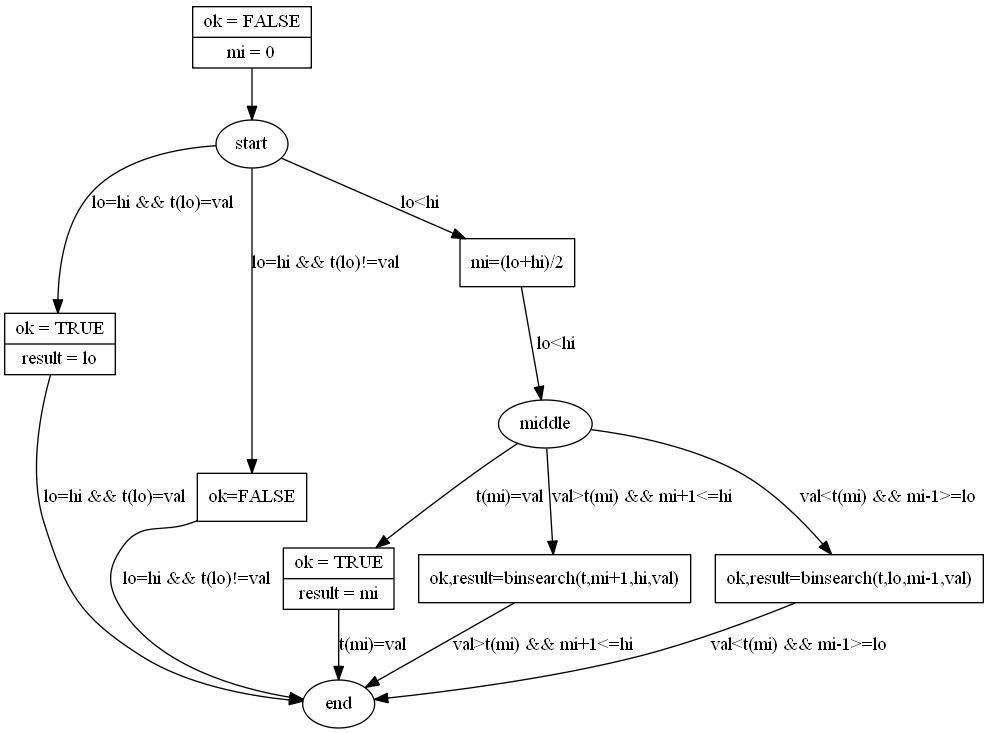
\includegraphics[width=0.8\textwidth]{img/pix.jpg}
  \caption{Visualized Representation of the Binary Search Algorithm}
  \label{fig:pix}
\end{figure}

Second, in Fig~\ref{fig:pix}, a textual representation of the binary search algorithm is given.
\begin{figure}[!h]
  \centering
    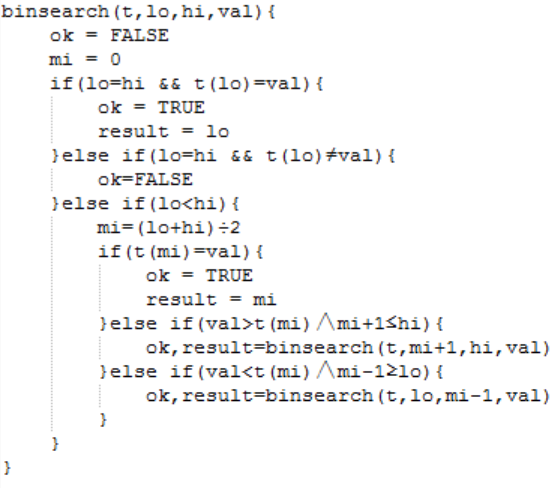
\includegraphics[width=0.5\textwidth]{img/alg.jpg}
  \caption{Textual Representation of the Binary Search Algorithm}
  \label{fig:alg}
\end{figure}








\end{document}

